\documentclass{standalone}
\usepackage{tikz}
\usetikzlibrary{quantikz}

\begin{document}

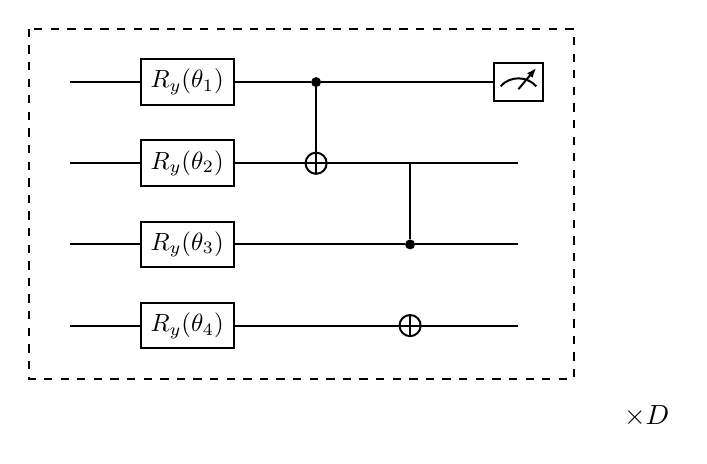
\begin{tikzpicture}
    \node[scale=0.9] {
        \begin{quantikz}[column sep=1cm]
            \lstick{} & \gate{R_{y}(\theta_1)} & \ctrl{1} & \qw & \meter{} \\
            \lstick{} & \gate{R_{y}(\theta_2)} & \targ{} & \qw & \qw \\
            \lstick{} & \gate{R_{y}(\theta_3)} & \qw & \ctrl{-1} & \qw \\
            \lstick{} & \gate{R_{y}(\theta_4)} & \qw & \targ{} & \qw
        \end{quantikz}
    };
    
    % Draw dashed box
    \draw[dashed, thick] ([xshift=-0.5em,yshift=0.5em]current bounding box.north west) rectangle ([xshift=0.5em,yshift=-0.5em]current bounding box.south east);
    
    % Add "× D" annotation
    \node[below right, xshift=0.5cm, yshift=-0.2cm] at (current bounding box.south east) {$\times D$};
\end{tikzpicture}

\end{document}